\chapter{Funções de Hash}
\label{cha:hash}

Uma função de hash mapeia uma sequência de bits de tamanho arbitrário em uma sequência curta e de tamanho fixo chamada {\em digest} ou {\em checksum}.
Em Estrutura de Dados estudamos funções de hash com o propósito de acessar uma lista em tempo $O(1)$.
Minimizar as colisões naquele contexto garantia que as listas ligadas de objetos associadas a cada índice de um vetor fosse a menor possível tornando a consulta mais eficiente.
Em aplicações de criptografia, evitar colisões é mais crítico, pois pode levar a vulnerabilidades no sistema.

Assim, uma função de hash é simplesmente uma função $H: \{0,1\}^* \to \{0,1\}^n$.
Para definir o conceito de resistência a colisão vamos introduzir artificialmete uma chave na função de hash que não precisa ser guardada em segredo.
Além disso, nosso modelo precisa conter além de $H$ um algoritmo $Gen$ que gera a chave.
O modelo, portanto, difere da construção prática.

Definiremos resistência à colisão para um sistema $\Pi = \langle Gen, H \rangle$ a partir do jogo que já nos abituamos:
\begin{enumerate}
\item O sistema usa $Gen$ que recebe $1^n$ e gera uma chave $s$.
\item O adversário $\mathcal{A}$ recebe $s$.
\item A devolve um par de mensagens $\langle x, x' \rangle$.
\end{enumerate}

O desafio de $\mathcal{A}$ é achar uma {\em colisão}, ou seja, um par $\langle x, x' \rangle$ tal que $H_s(x) = H_s(x')$
\begin{displaymath}
  HashCol_{\mathcal{A}, \Pi}(n) := \left\{
    \begin{array}{lcl}
      1 & \textrm{se} & H_s(x) = H_s(x')\\
      0 & \textrm{c.c.} &\\
    \end{array}
    \right.
\end{displaymath}

O sistema $\Pi$ é {\em resistente à colisão} \cite{Damgard88} se para todo adversário polinomial $\mathcal{A}$ existe uma função desprezível $\varepsilon$ tal que:
\begin{displaymath}
  Pr[HashCol_{\mathcal{A}, \Pi}(n) = 1] \leq \varepsilon(n)
\end{displaymath}

A necessidade de inserir uma chave é puramente técnica.
Sem uma chave não seria possível evitar que o adversário simplesmente pré-compute uma colisão e use-a para derrotar o jogo.
Na prática usamos funções sem chave e tratamos como resistentes a colisão quando isso for validade empiricamente.

Note que a resistência à colisão é uma propriedade mais forte do que outras propriedades desejáveis em funções de hash:
\begin{itemize}
\item {\em resistência contra colisões em alvos específicos}: dado $s$ e $x$ nenhum adversário eficiente é capaz de encontrar $x'$ tal que $H_s(x) = H_s(x')$ com probabilidade considerável.
\item {\em resistência contra preimagem}: dados $s$ e $y$ aleatório, nenhum adversário eficiente é capaz de encontrar $x$ tal que $h_s(x) = y$ com probabilidade considerável. 
\end{itemize}

Toda a função de hash está sujeita a ataques do tipo força bruta.
Ou seja, se $H: \{0,1\}^* \to \{0,1\}^n$ podemos calcular $H(x)$ para uma sequência de strings distintas $x_0, x_1, \dots, x_{2^n+1}$.
Pelo {\em princípio da casa dos pombos} necessariamente encontraremos neste caso uma colisão.
Na verdade se assumirmos que $H$ é uma função aleatória, podemos mostrar que para que a probabilidade de encontrar uma colisão seja maior do que $\frac{1}{2}$ precisamos nossa sequência strings deve ter cerca de $\Theta(\sqrt{n})$.
Esse resultado é chamado de {\em paradoxo do aniversário}, pois bastam 23 pessoas para garantir que a probabilidade de duas fazerem aniversário no mesmo dia seja maior que meio.
Assim, se quisermos um sistema que garanta a segurança equivalente a uma função aleatória com chave de 128 bits, precisamos usar uma função de hash muito confiável que produz uma saída com pelo menos 256 bits.

O ataque do aniversariante nos dá uma colisão qualquer $\langle x, x' \rangle$ a primeira vista isso pode parecer inofencivo, pois não podemos controlar os valores de $x$ e  $x'$.
Note, porém, que o ataque requer uma serie de pelo menos $\sqrt{n}$ mensagens, mas elas não precisam ser aleatórias.
Precisamos, portanto, apenas gerar um número suficente de mensagens equivalentes para que o ataque seja efetivo.
Essa é uma tarefa relativamente simples.
Considere o seguinte exemplo de um conjunto de mensagens equivalentes:


\begin{quote}
  É {\em difícil/impossível/desafiador/complicado} {\em imaginar/acreditar} que {\em encontraremos/localizaremos/contrataremos} outra {\em pessoa/empregada} com a mesma {\em capacidade/versatilidade/destreza} que Eva.
Ela fez um trabalho {\em incrível/excelente}.
\end{quote}

% mudar esse exemplo que está identico ao do livro

As palavras em itálico podem umas substituir as outras sem mudar significativamente o espírito da mensagem que pode ser escrita de 288 formas distintas.
Se nosso conjunto precisa ser $2^{32}$ basta escrever um texto com pelo menos 32 palavras em que cada uma possua um sinônimo.
 
\section{Construções}
\label{sec:construcoes}

A maioria das funções de hash seguem uma construção chamada {\em Merkle-Damgard} que assume a existância de uma {\em função de compressão} resistente à colisão para mensagens de tamanho fixo e a extende para mensagens de tamanho arbitrário \cite{Merkle89,Damgard89}.
Seja $\langle Gen, h \rangle$ um sistema de hash que comprime o tamanho de uma mensagem pela metade $h_s:\{0,1\}^{2n} \to \{0,1\}^n$.
Construimos $\langle Gen, H \rangle$ da seguinte maneira:
\begin{itemize}
\item Sejam $x \in \{0,1\}^*$, $|x| = L < 2^n$ e $B := \lceil \frac{L}{n} \rceil$ o número de blocos de $x$ de tamanho $n$ (se o tamanho de $x$ não for múltiplo de $n$ complete-o com um {\em pad} de $0$s) e insira $L$ ao fim de $x$ i.e. $x = x_0 \dots x_B L$.
\item Defina $z_0 := 0^n$.
\item Compute $z_i := h_s(z_{i-1}x_i)$ para $i = 1, \dots, B + 1$.
\item Devolva $z_{B+1}$.
\end{itemize}

\begin{figure}[htbp]
  \centering
    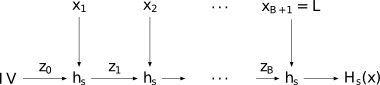
\includegraphics[width=.5\textwidth]{imagens/Merkle-Damgard.png}
  \caption{Diagrama da construção de Merkel Damgrad}
  \label{fig:merkle-damgard}
\end{figure}


\begin{theorem}[Merkle-Damgard]
  Se $\langle Gen, h \rangle$ é resistente a colisão então $\langle Gen, H \rangle$ da forma como definido acima também é resistente a colisão.
\end{theorem}

Construir uma função de hash resistente a colisão para uma mensagem de tamanho arbitrário se resume, portanto, a encontrar uma para mensagem de tamanho fixo que a comprima pela metade.

\subsection{SHA-1}
\label{sec:sha-1}

O {\em Secure Hash Algorithm} (SHA-1) é um algoritmo da família MD4 que recebe uma entrada de tamanho arbitrário $l < 2^{64}$ e produz um {\em digest} de $160$ bits.
Antes de processar a mensagem é inserido um {\em pad} que consiste em uma sequência $10 \dots 0l$ em que $l = |x|$ é o número de bits da mensagem e $|x10 \dots 0l|$ é um múltiplo de 512.
Essa codificação de $x$ é então dividida em blocos $x_0, \dots, x_n$ tais que $|x_i| = 512$.

A função de hash $h$ que alimenta a construção de Merkle-Damgard consiste de 80 rodadas.
Um {\em message schedule} é responsavel por gerar 80 strings $W_0, \dots, W_{79}$ de 32 bits cada a partir do bloco $x_i$ sendo processado. 
Começamos com valores iniciais fixos $A =$ {\tt 67452301}, $B =$ {\tt EFCDAB89}, $C =$ {\tt 98BADCFE}, $D =$ {\tt 10325476}, $E =$ {\tt C3D2E1F0} e alteramos esses valores em cada rodada da seguinte maneira:

\begin{displaymath}
  A, B, C, D, E := (E + f_t(B,C,D) + A_{\lll 5} + W_j + K_t), A, B_{\lll 30}, C, D
\end{displaymath}

A cada 20 rodadas mudamos o valor da constante $K_t$ e da função $f_t$ de forma que o algoritmo precisa definir 4 constantes e quatro funções.
Apenas para matar a curiosidade seguem suas definições:
\begin{enumerate}
\item $K_t :=$ {\tt 5A827999} e $f_t(B,C,D) := (B \land C) \lor (B \land D)$ para $t = 0, \dots, 19$
\item $K_t :=$ {\tt 6ED9EBA1} e $f_t(B,C,D) := B \xor C \xor D$ para $t = 20, \dots, 39$ 
\item $K_t :=$ {\tt 8F1BBCDC} e $f_t(B,C,D) := (B \land C) \lor (B \land D) \lor (C \land D)$ para $t = 40, \dots, 59$
\item $K_t :=$ {\tt CA62C1D6} e $f_t(B,C,D) := B \xor C \xor D$ para $t = 60, \dots, 79$ 
\end{enumerate}

Em fevereiro de 2017 um grupo de pesquisadores da Google e de uma faculdade holandesa anunciaram um ataque prático contra o SHA-1 capaz de encontrar colisões\footnote{https://security.googleblog.com/2017/02/announcing-first-sha1-collision.html}.
Os autores estimaram que um ataque força-bruta em uma ano requereria cerca de 12 milhões de processadores gráficos para encontrar uma colisão, mas explorando as vulnerabilidades apontadas isso pode ser executado com apenas 110 processadores.
Como prova do conceito eles produziram dois documentos PDF com um infográfico explicando sobre o ataque.
Cada um desses arquivos possui uma cor diferente, mas ambos produzem o mesmo hash quando processados pelo SHA-1.
A orientação hoje é utilizar sistemas de hash mais seguros como o SHA-256 e o SHA-3.

\section{Aplicações}
\label{sec:aplicacoes}

Funções de hash são amplamente utilizadas em protocolos de segurança.
Nesta seção veremos quatro aplicações bastante distintas desses sistemas: um sistema de autenticação bastante popular chamado HMAC, identificação de arquivos e outros tipos de mensagens simples e estruturadas  ({\em fingerprints} e {\em árvore de Merkle}) e derivação de subchaves a partir de outras chaves e a partir de uma senha.

\subsection{HMAC}
\label{sec:hmac}

No capítulo anterior vimos como construir um sistema de autenticação para mensagens de tamanho arbitrário aplicando um esquema similar ao modo CBC.
Alternativamente poderíamos utilizar um hash para produzir um {\em digest} da mensagem de tamanho fixo e então aplicar um sistema de autenticação para mensagens de tamanho fixo no resultado.
Esse sistema é conhecido como {\em Hash-and-MAC}.

Considere um sistema de autenticação $\Pi_M = \langle Gen_M, Mac_M, Ver_M \rangle$ para mensagens de tamanho fixo $l(n)$ e um sistema de hash $\langle Gen_H, H \rangle$ que produz um {\em digest} de tamanho $l(n)$.
O sistema {\em Hash-and-MAC} $\Pi = \langle Gen, Mac, Ver \rangle$ para mensagens de tamanho arbitrário é definido como:
\begin{itemize}
\item $Gen(1^n) := k = \langle k_M, s \rangle$ em que $Gen_M(1^n) := k_M$ e $Gen_H(1^n) := s$
\item $Mac(k, m) := Mac_M(k_M, H_s(m))$
\item $Ver(k, m, t) := \left\{
    \begin{array}{lcl}
      1 & \textrm{se} & Mac(k,m) = t\\
      0 & \textrm{c.c.} &\\
    \end{array}
    \right.$ 
\end{itemize}


\begin{theorem}
  Se $\Pi_M$ é um sistema de autenticação seguro contra falsificação e $\Pi_H$ é um sistema de hash resistente a colisão então a construção $\Pi$ acima é seguro contra falsificação. 
\end{theorem}

\begin{proof}
  Vamos apenas esboçar a prova e deixar os detalhes para o leitor.
  A ideia é a seguinte, suponha que o adversário $\mathcal{A}$ consulte o tag de uma série de mensagens $Q$ e então suponha por absurdo que ele consiga produzir um código válido para uma mensagem $m \notin Q$.
  Neste caso temos duas possibilidades:
  \begin{enumerate}
  \item existe uma mensagem $m' \in Q$ tal que $H_s(m') = H_s(m)$, mas isso contradiz a hipótese que $\Pi_H$ é resistente a colisões
  \item caso contrário $\mathcal{A}$ conseguiu falsificar um código para uma mensagem nova $H_s(m)$ de tamanho $l(n)$ contradizendo a hipótese que $\Pi_M$ é seguro contra falsificação.
  \end{enumerate}
\end{proof}

O popular sistema de autenticação HMAC se inspira no esquema apresentado acima usando duas vezes uma função de hash e duas constantes distintas {\tt ipad} e {\tt opad}.
Formalmente definimos o sistema HMAC da seguinte forma:
\begin{itemize}
\item $Gen(1^n) := k \leftarrow \{0,1\}^n$
\item $Mac(k, m) := H_s((k \xor \textrm{\tt opad}) || H_s(k \xor \textrm{\tt ipad})m)$
\item $Ver(k, m, t) := \left\{
    \begin{array}{lcl}
      1 & \textrm{se} & Mac(k,m) = t\\
      0 & \textrm{c.c.} &\\
    \end{array}
    \right.$
\end{itemize}

% argumentar sobre a importância das duas constantes e a relação com o sistema anterior

\subsection{Fingerprints e Árvores de Merkle}
\label{label}

Um hash seguro contra colisão pode ser usado para identificar um arquivo ou uma mensagem qualquer de maneira eficiente.
Esse identificador costuma ser chamado de {\em fingerprint} ou impressão digital do arquivo.
Fingerprints são utilizados em diversas aplicações como para identificação de malwares, para encontrar arquivos duplicados em um HD, para encontrar um arquivo em uma rede P2P (um {\em link magnético} nada mais é do que um fingerprint de um arquivo) e para verificar chaves (veremos isso no Capítulo \ref{cha:protocolos}).

Considere agora a situação em que temos uma série de $n$ arquivos em um servidor e gostaríamos de identificá-los localmente para verificar se o arquivo recuperado não foi corrompido.
Uma solução simples seria guardar localmente um fingerprint de cada um dos arquivos.
Essa solução requer o armazenamento e gerenciamento de $n$ fingerprints.
Uma solução mais eficiente é usar uma {\em árvore de Merkle}.
Uma árvore de Merkle é uma árvore binária em que as folhas são os arquivos e cada nó é o hash dos seus dois filhos.
Assim podemos armazenar localmente apenas o valor da raiz da árvore.
Toda vez que recuperarmos um arquivo o servidor deve enviar uma prova de que o arquivo não foi corrompido.
Essa prova consiste dos valores da árvore de Merkle no caminho da raíz até a folha (note que são necessários $lg(n)$ valores).
Com isso locamente conseguimos recuperar o valor da raíz e comparar com o que armazenamos localmente.
Veremos no Capítulo \ref{cha:protocolos} como as árvores de Merkle são usadas nos protocolos de criptomoeadas.

\subsection{Funções de Derivação de Chaves}
\label{sec:kdf}

Uma {\em função de derivação de chaves} (KDF) tem como objeto produzir uma chave segura a partir de algum material contendo uma boa quantidade de entropia chamado {\em key material}.
Isso pode ser útil seja porque o {\em key material} não está suficientemente preparado para ser usado como uma chave -- por exemplo no caso de uma senha -- ou quando queremos derivar {\em subchaves} a partir de uma chave inicial.

Formalmente, uma função de derivação de chaves recebe com entrada o {\em key material} $\delta$, o tamanho $l$ da chave a ser produzida e opcionalmente um valor $r$ chamado de {\em salt} e um valor contextual $c$.
Um KDF seguro deve produzir a partir desses valores uma sequência {\em pseudoaleatória} de tamanho $l$.
Tipicamente um KDF consiste de duas etapas: 
\begin{enumerate}
\item {\em extração}: recebe o {\em key material} e opcionalmente uma chave pública ({\em salt}) e produz uma sequência pseudoaleatória de bits de tamanho fixo
\item {\em expansão}: expande o que foi produzido na fase de extração para uma sequência de bits de tamanho $l$.
\end{enumerate}

Uma implementação popular deste modelo é o HKDF \cite{Krawczyk10} que usa apenas o HMAC como primitiva:

\begin{eqnarray*}
  \textrm{PRK}      & := & \textrm{HMAC}(r, \delta)\\
  \textrm{HKDF}(r, \delta, c, l) & := & K(1)||K(2) \dots ||K(t)\\
  K(1)     & := & \textrm{HMAC}(\textrm{PRK}, c||0)\\
  K(i + 1) & := & \textrm{HMAC}(\textrm{PRK}, K(i)||c||i)\\
\end{eqnarray*}

No caso $\delta$ seja uma senha proposta por um usuário, temos um problema a mais, pois tipicamente essas possuem uma entropia baixa e, portanto, estão sujeitas a {\em ataques de dicionário}.
Para mitigar este problema podemos utilizar uma função de derivação de chaves lenta.
Um {\em password based key derivation function} recebe como parâmetro, além do salt $r$, do tamanho $l$ e da senha $\delta$, um valor que estipula o número de ciclos $n$.
Uma implementação popular deste modelo é o PBKDF2:

\begin{eqnarray*}
  \textrm{PBKDF2}(r, \delta, c, n, l) & := & K(1)||K(2)|| \dots ||K(t)\\
  K(i)     & := & U_0^i \xor U_1^i \xor \dots \xor U_n^i\\
  U_0^i    & := & H(\delta||r||i)\\
  U_j^i    & := & H(\delta||U_{j-1}^1)\\
\end{eqnarray*}

Note que a primitiva neste caso é uma função de hash $H$ e que cada $K(i)$ roda $n$ vezes essa função.
O salt impede o preprocessamento de um dicionário e $n$ deve ser grande o suficiente para impedir sua construção {\em a posteriori}.


\section{Exercícios}
\label{sec:exercicios}


\begin{exercicio}
  Mostre que resistência contra colisões garante a resistência contra preimagem.
\end{exercicio}

\begin{exercicio}
  Mostre que o seguinte sistema não é seguro contra falsificação considerando que o sistema de hash foi construído a partir do paradigma de Merkle-Damgard:
\begin{itemize}
\item $Gen(1^n) := k \leftarrow \{0,1\}^n$
\item $Mac(k,m) := H(k||m)$
\item $Ver(k,m,t) := \left\{
    \begin{array}{lcl}
      1 & \textrm{se} & Mac(k,m) = t\\
      0 & \textrm{c.c.} &\\
    \end{array}
    \right.$ 
\end{itemize}
\end{exercicio}

\begin{exercicio}
% arvores de Merkle
\end{exercicio}

